
\chapter{Erstes Kapitel}
Schön ist, wenn man als Leser in das Kapitel eingeführt wird, bevor
der nächste Unterabschnitt (hier \ref{abs:erster}) folgt.

\section{Ein Abschnitt}\label{abs:erster}
Hier steht dann so BlaBla zum Thema.

\subsection{Ein Unterabschnitt}
Mit etwas Text

\paragraph{Eine Zwischenüberschrift}
Auch mit etwas mehr Text

\subsection{Ein weiterer Unterabschnitt}\label{abs:naja}
Text

% Eine Vektorgrafik (eps) einfügen...
\begin{figure}[ht!]
 \centering
 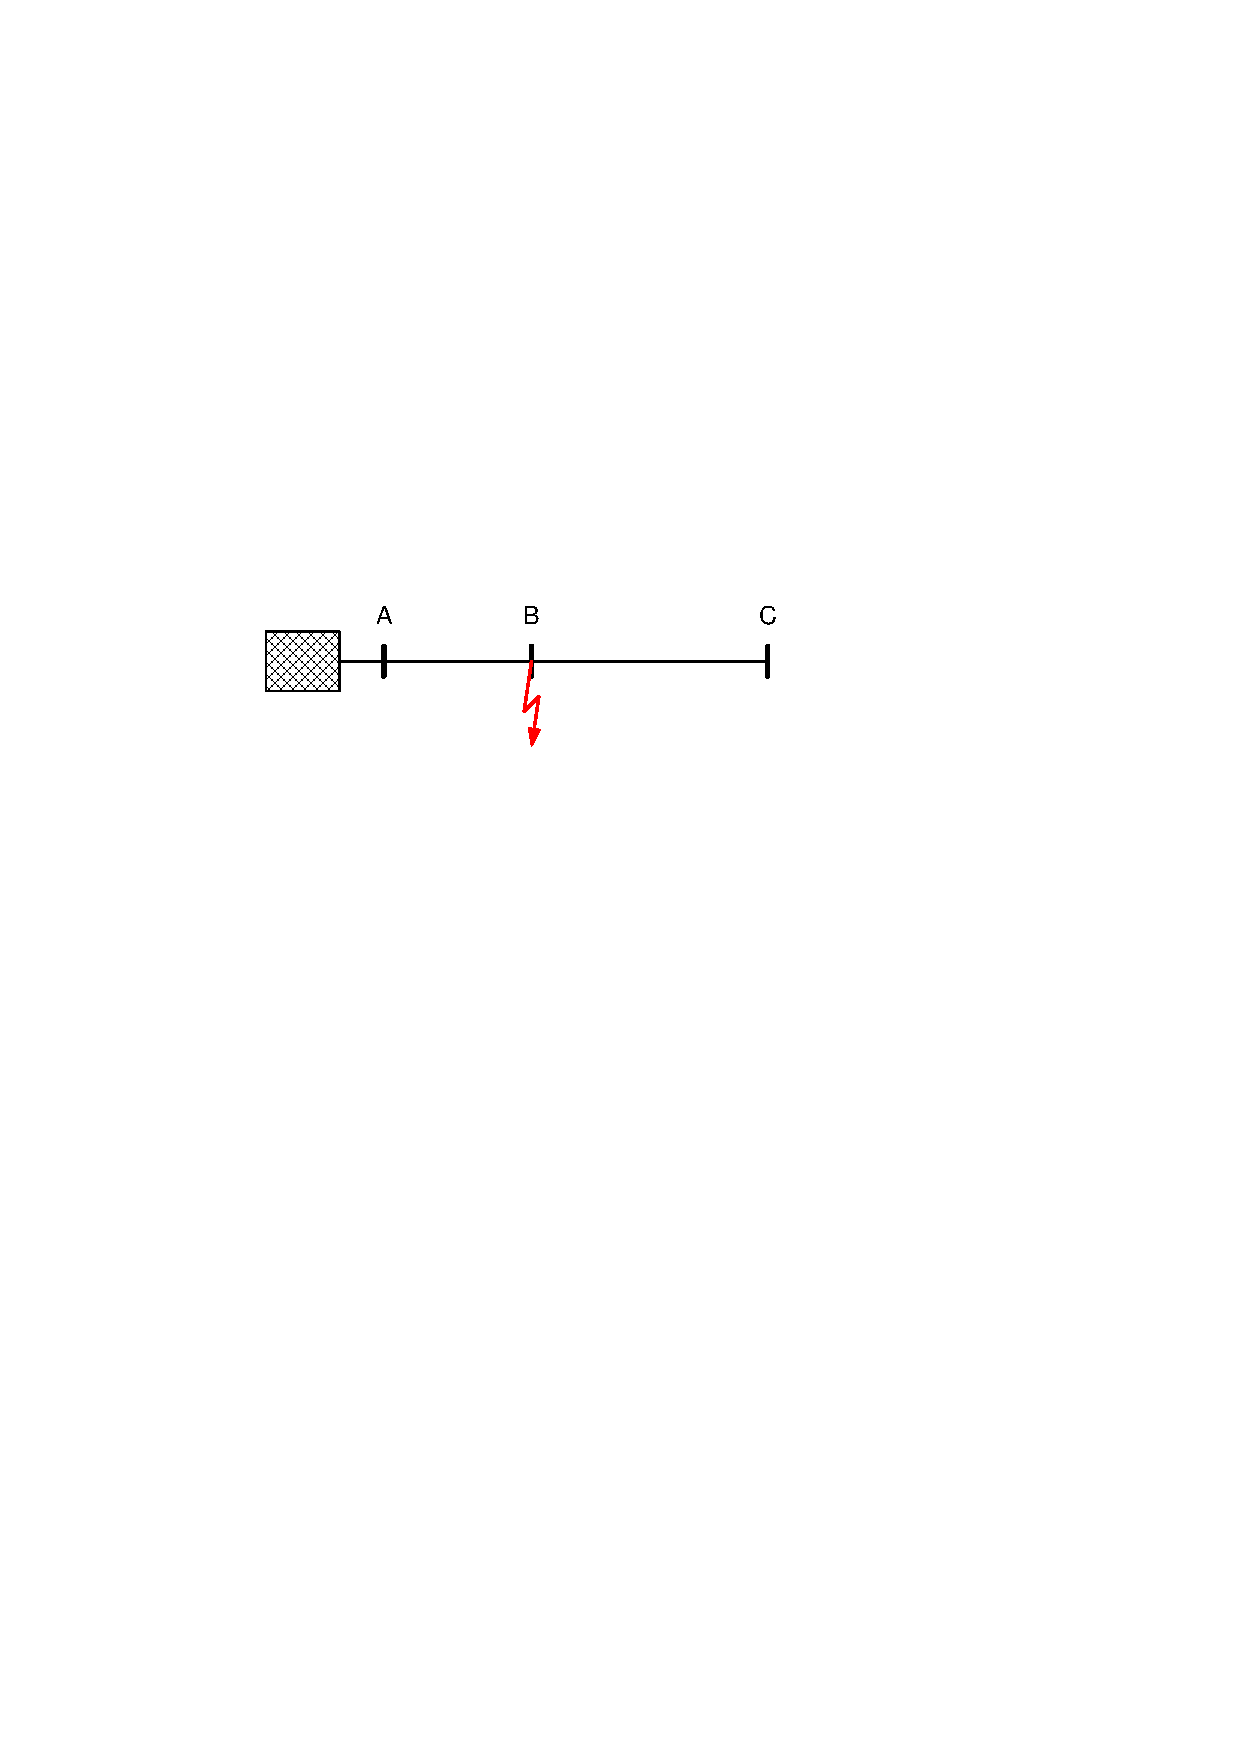
\includegraphics[width=.6\textwidth]{Inhalt/Abbildungen/Bild_Visio.pdf}
 % Bildunterschriften immer unter dem Bild
 \caption{Schematisches Netzmodell für Simulationen --- Bilder haben immer Unterschriften}
 \label{fig:leitungsmodell}
\end{figure}

% Eine Tabelle...
% Bei sehr langen Tabellen das Paket "longtable" verwenden!
\begin{table}[ht!]
 \centering
 % Tabellenbeschriftung immer über der Tabelle
 \caption{Liste der Zustände --- Tabellen haben immer Überschriften}
 \label{tab:Zustaende}
 \begin{tabular}{|r|r|r|l|}
   \hline
   Aufeinanderfolgende & Sollwert\_1: & Sollwert\_2: & Weiterschaltbedingung: \\
   Zustandsnummern: & & & \\
   \hline
   100 & 0 & 0 & Zeitgeber \SI{50}{ms} \\
   10 & 10 & 0 & Istgeschwindigkeit\_1 = 10\\
   20 & 0 & 20 & Zeitgeber \SI{100}{ms} \\
   30 & -10 & 20 & Istgeschwindigkeit\_1 = 0 \\
   40 & 0 & 0 & Zeitgeber $\SI{50}{\micro s}$ \\
   50 & -15 & 0 & Istgeschwindigkeit\_1 = -15 \\
   60 & 0 & -20 & Zeitgeber $\SI{50}{ms}$ \\
   \hline
  \end{tabular}
\end{table}

\pagebreak	% manueller Seitenumbruch (Fall's das mal wirklich
                % sein muss; möglichst LaTeX machen lassen und solche
                % Befehle vermeiden!)

\section{Neuer Abschnitt}

% Mehrere Gleichungen...
\begin{eqnarray}
\K{u}_1 = R_1 \, \K{i}_1 + \frac{d \, \K{\Psi}_\bez{res}}{dt} \quad \Rightarrow&
\underbrace{\K{u}_1 = R_1 \, \K{i}_1 + \bez{j} \, \omega \, w_\bez{eff} \, \K{\Phi}_h}  \\
 & \text{eingeschwungener Zustand} \nonumber
\end{eqnarray}

% Inline-Gleichungen (also Formelzeichen im Text)...
Hierbei ist $R_1$ der Ständerwiderstand, $\K{\Psi}_\bez{res}$ der
resultierende Fluss der Maschine und $w_\bez{eff}$ die wirksame
Windungszahl.
% Eine einzige Gleichung...
\begin{equation}
 \K{\Phi}_h \, \omega w_\bez{eff} = \K{i}_1 \, L_1 \quad \Rightarrow  \quad
 \K{i}_1 = \frac{\K{u}_1}{R_1 + \bez{j} \, \omega \, L_1}
\label{eqn:is}
\end{equation}

% Tabelle, die Formelzeichen verdeutlicht ...
\begin{table}[ht!]
 \centering
 % Tabellenbeschriftung immer über der Tabelle
 \caption{Richtige Formelzeichen sind eine Kunst für sich \dots \cite{din1303,din1304}}
 \label{tab:Formelzeichen}
 \begin{tabular}{|c|l|l|}
   \hline
   Formelzeichen & Bedeutung und Hinweise \\
   \hline
   $I$, $k$ & Variablen (Skalare) werden kursiv geschrieben \\
   $\imag$, $\SI{}{\Omega}$, $\SI{}{A}$ & die imaginäre Einheit mit $\backslash$\texttt{imag} ist wie alle Einheiten\footnotemark aufrecht \\
   $\upmu_0$, $\upepsilon_0$ & auch Konstanten werden aufrecht geschrieben \\
   $\K{I}$ & komplexe Größen sind unterstrichen \\
   $\VM{i}$ & Vektoren (Zeilen- oder Spaltenvektor) sind klein, fett und kursiv \\
   $\VM{R}$ & Matrizen sind groß, fett und kursiv \\
   $\KVM{Z}$ & \dots natürlich kombinierbar auch mit komplexen Größen \\
   $I_\bez{max}$, $I_\bez{k}^{''}$,  & Bezeichnungen als Indizes sind nicht kursiv \\
   $I_{k}$ mit $k=1,2,\dots$ & \dots (Zähl)variablen aber schon \\
   $Z_{1,3}$ $\leftrightarrow$ $Z_{k\,l}$, $i^{''}_{\bez{k}\:\max}$  & \textbf{nur} Matrizenindizes werden durch Komma getrennt \\
   \hline
  \end{tabular}
\end{table}
\footnotetext{Zahlen mit Einheiten am besten mit einem Paket wie \emph{units} oder \emph{sistyle} setzten.}

\section{Referenzen}
% Jetzt kommen Hinweise, wie Querverweise auf Gleichungen, Tabellen,
% usw. erzeugt werden.
In Gleichung~(\ref{eqn:is}) wird \dots \\
Dagegen ist in Tabelle~\ref{tab:Zustaende} ist nur Mist dargestellt
und das Bild~\ref{fig:leitungsmodell} auf
Seite~\pageref{fig:leitungsmodell} in Abschnitt~\ref{abs:naja} sagt
auch nicht viel aus. Also macht es in Eurer Diplom- bzw. Studienarbeit
besser!

\section{Hinweise}
Für \LaTeX-Literatur ist Helmut Kopka's Buch \cite{kopka} sehr zu
empfehlen und auch zahlreich in der SLUB vorhanden. Als Editor unter
Windows kann ich den \LaTeX-Editor \cite{led} wärmstens
empfehlen. Damit der eingebaute DVI-Betrachter auch richtig
funktioniert, muss das Microsoft~.NET-Framework 2.0 installiert sein.